\chapter{连续状态演化、流、采样与离散时间模型}

%——————————————————————————————————%

\newenvironment{dynamicscase}[1]{%
    \par\noindent\textbf{\color{main}例：#1}\rmfamily\par
}{%
    \par\ignorespacesafterend
}

前面的章节建立了从拓扑、流形到切空间和向量场的连续几何语言。本章补上从这套语言进入机器人算法时最容易被省略的一层：真实系统在连续时间中演化，而传感器和计算机只能在离散时刻读取数据、保存状态并进行数值计算。

这里必须区分三个不同层次：
\[
\begin{array}{ccl}
    x(t) &:& \text{连续时间的真实状态},\\
    x_k=x(t_k) &:& \text{真实轨迹在采样时刻的状态},\\
    \hat{x}_k &:& \text{算法在第 }k\text{ 个时刻维护的数值估计}.
\end{array}
\]
它们满足的基本关系是
\[
    x(t)\in M,\qquad x_k\in M,\qquad \hat{x}_k\in M,
\]
其中$M$是状态空间。时间和计算步骤被离散化，并不意味着状态空间本身被替换成有限个格子。即使算法只保存$\{\hat{x}_k\}$，每一个估计仍然是连续流形$M$上的一个点。

本章的主线是
\[
\begin{aligned}
    &\text{状态曲线}
    \longrightarrow \text{切向量与向量场}
    \longrightarrow \text{连续时间ODE与积分曲线}\\
    &\longrightarrow \text{流}
    \longrightarrow \text{采样}
    \longrightarrow \text{离散状态转移}\\
    &\longrightarrow \text{数值近似}
    \longrightarrow \text{观测模型与离散时间状态空间模型}.
\end{aligned}
\]
这条链回答一个核心问题：连续时间、流形上的真实运动，如何成为离散时刻、仍然位于同一状态流形上的状态序列？

本章只建立桥梁，不展开Kalman滤波、IMU预积分、随机微分方程、因子图或高阶数值积分。它们都需要本章的对象和映射类型作为前提。

%——————————————————————————————————%

\section{真实状态是流形上的连续曲线}

\subsection{状态、轨迹与瞬时速度}

设$M$是一个光滑流形。机器人在时间区间$I\subseteq\R$内的真实状态轨迹是一个映射
\[
    x:I\to M,
    \qquad
    t\longmapsto x(t).
\]
在每一个时刻$t$，状态$x(t)$是$M$中的一个点；它不是一组已经选定的欧氏坐标。

由第五章的曲线切向量定义，轨迹在$t$处的瞬时速度是
\[
    \dot{x}(t)\in T_{x(t)}M.
\]
这里的下标非常重要：速度属于当前状态点的切空间，而不是一个与所有状态点共享的固定向量空间。

\begin{definition}[向量场]
流形$M$上的向量场$X$是在每个$p\in M$指定一个切向量$X_p\in T_pM$的光滑规则，记为
\[
    X\in\Gamma(TM),
    \qquad
    p\longmapsto X_p.
\]
\end{definition}

如果状态演化由一个自治向量场规定，则连续时间动力学写成
\[
    \dot{x}(t)=X_{x(t)}.
\]
等式两边都属于$T_{x(t)}M$，所以这是一个类型正确的内蕴表达。

若系统还受到控制输入$u(t)\in\mathcal U$影响，则动力学可以写为
\[
    \dot{x}(t)=f(x(t),u(t)),
    \qquad
    f(x,u)\in T_xM.
\]
严格地说，$f$不是一个任意取值于某个固定$\R^n$的函数，而是满足
\[
    f:M\times\mathcal U\to TM,
    \qquad
    \tau_M(f(x,u))=x
\]
的映射，其中$\tau_M:TM\to M$是切丛投影。固定一个输入$u$后，$f(\mathord\cdot,u)$就是状态流形上的一个向量场。

\begin{center}
\begin{tikzpicture}[>=stealth]
    \node (time) at (0,1.7) {$t\in I$};
    \node (state) at (4,1.7) {$x(t)\in M$};
    \node (velocity) at (4,0) {$\dot{x}(t)\in T_{x(t)}M$};
    \draw[->] (time) -- node[above] {$x$} (state);
    \draw[->] (time) -- node[right] {$\dot{x}$} (velocity);
    \draw[->] (state) -- node[right] {$\text{所在点决定切空间}$} (velocity);
\end{tikzpicture}
\end{center}

\begin{dynamicscase}{三个容易混淆的对象}
在同一个状态流形$M$上，
\[
\begin{array}{c|c|c}
\text{对象} & \text{所在空间} & \text{含义}\\ \hline
x(t) & M & \text{时刻 }t\text{ 的状态点}\\
\dot{x}(t) & T_{x(t)}M & \text{该状态处的瞬时速度}\\
X & \Gamma(TM) & \text{在整个状态空间上给出速度的规则}\\
X_{x(t)} & T_{x(t)}M & \text{向量场在当前状态处的取值}
\end{array}
\]
因此不能把$X$、$X_{x(t)}$和$\dot{x}(t)$当作同一个对象。若轨迹由$X$生成，则它们通过$\dot{x}(t)=X_{x(t)}$联系起来。
\end{dynamicscase}

\subsection{局部坐标中的ODE}

取一张包含$x(t_0)$的坐标图$(U,\varphi)$。在轨迹仍留在$U$的时间区间内，连续状态曲线可写成欧氏坐标曲线
\[
    \bar{x}(t):=\varphi(x(t))\in\varphi(U)\subseteq\R^n.
\]
在这套坐标下，向量场和动力学有一个普通的分量表达：
\[
    \frac{d}{dt}\bar{x}(t)
    =\bar{f}(\bar{x}(t),u(t)).
\]
换一张坐标图时，$\bar{x}$和$\bar{f}$都会按照坐标转换的Jacobian变换。可微结构保证这些局部表达描述的是同一个内蕴动力学，而不是两套互不相容的方程。

这里也可以看出第五章之前各个概念的分工：状态是流形上的点，速度是切向量，向量场负责给出每个点的速度，而局部坐标只负责把它们转换为可以计算的欧氏分量。

%——————————————————————————————————%

\section{从向量场到积分曲线与流}

\subsection{积分曲线}

\begin{definition}[积分曲线]
给定光滑向量场$X\in\Gamma(TM)$，一条曲线$\gamma:I\to M$称为$X$的积分曲线，如果
\[
    \dot{\gamma}(t)=X_{\gamma(t)},
    \qquad t\in I.
\]
若还给定初始状态$p\in M$，则通常要求
\[
    \gamma_p(0)=p.
\]
\end{definition}

积分曲线的图像是：向量场在每个位置放置一根瞬时速度箭头，轨迹始终沿着当前位置的箭头运动。它把“每个点允许怎样动”的局部规则，整合成一条随时间变化的全局轨迹。

在局部坐标中，这一定义退化为常微分方程初值问题。若$X$足够光滑，则局部存在性与唯一性定理保证：对每个初始状态$p$，至少在$t=0$附近存在唯一积分曲线。若轨迹在有限时间内不会离开定义域，并且可以延拓到所有时间，则称$X$是完备的。

\subsection{流映射}

只要初值问题的解在所需时间存在，就可以把每个初始点$p$送到它演化$t$时间后的状态：
\[
    \Phi_t(p):=\gamma_p(t).
\]
这里$\Phi_t$可能只是定义在$M$的某个开子集上；当向量场完备时，对每个$t\in\R$都可以得到全局映射$\Phi_t:M\to M$。

\begin{definition}[流]
由自治向量场$X$生成的流是一族映射$\{\Phi_t\}$，满足
\[
    \Phi_0=\operatorname{id}_M,
    \qquad
    \Phi_{s+t}=\Phi_s\circ\Phi_t,
\]
并且$\Phi_t(p)$是从$p$出发沿$X$运动$t$时间的状态。
\end{definition}

第二条关系来自时间演化的可组合性：先演化$t$时间，再演化$s$时间，与一次性演化$s+t$时间相同。注意复合顺序：对$p$先作用的是右侧的$\Phi_t$，所以
\[
    (\Phi_s\circ\Phi_t)(p)=\Phi_s(\Phi_t(p)).
\]

\begin{center}
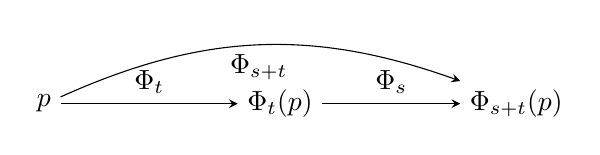
\begin{tikzpicture}[>=stealth]
    \node (p) at (0,1.7) {$p$};
    \node (pt) at (3,1.7) {$\Phi_t(p)$};
    \node (pst) at (6,1.7) {$\Phi_{s+t}(p)$};
    \draw[->] (p) -- node[above] {$\Phi_t$} (pt);
    \draw[->] (pt) -- node[above] {$\Phi_s$} (pst);
    \draw[->,bend left=22] (p) to node[below] {$\Phi_{s+t}$} (pst);
\end{tikzpicture}
\end{center}

\begin{proposition}[流的逆映射]
在流定义良好的时间范围内，
\[
    \Phi_{-t}\circ\Phi_t=\operatorname{id}_M,
    \qquad
    \Phi_t\circ\Phi_{-t}=\operatorname{id}_M.
\]
因此$\Phi_t$的逆映射是$\Phi_{-t}$。若$X$是完备光滑向量场，则每个$\Phi_t$都是$M$上的微分同胚。
\end{proposition}

流把连续动力学压缩成了一个状态转移映射：输入一个状态$p$和一个时间长度$t$，输出演化后的状态$\Phi_t(p)$。第五章李群中的指数曲线正是这一思想在李群上的特殊情形。

\subsection{有输入时的时间转移}

若动力学显含输入$u(t)$，则同一个向量场不再固定不变。给定输入轨迹$u(\mathord\cdot)$和起止时刻$s\le t$，记对应的状态转移为
\[
    \Phi^u_{t,s}:M\to M.
\]
它把初始状态$x(s)$送到由输入$u(\tau)$驱动、在$t$时刻得到的状态$x(t)$：
\[
    x(t)=\Phi^u_{t,s}(x(s)).
\]
不同区间的转移仍然可以复合：
\[
    \Phi^u_{t_2,t_1}\circ\Phi^u_{t_1,t_0}
    =\Phi^u_{t_2,t_0},
    \qquad t_0\le t_1\le t_2.
\]
与自治流不同，这里的转移通常不只由时间差$t-s$决定，还依赖区间上的完整输入轨迹。

%——————————————————————————————————%

\section{欧氏空间中的连续模型}

\subsection{切空间的自然识别}

当$M=\R^n$时，每个点的切空间都可以通过平移自然识别为
\[
    T_x\R^n\simeq\R^n.
\]
因此熟悉的欧氏常微分方程
\[
    \dot{x}(t)=f(x(t),u(t)),
    \qquad x(t)\in\R^n,
\]
在类型上没有明显的区别：状态和速度都可以用$n$个实数组成的列向量表示。但这只是线性空间的特殊便利，不能直接推广到任意流形。

\subsection{一个可以精确离散的例子}

考虑一维受控粒子：
\[
    x(t)\in\R,
    \qquad
    \dot{x}(t)=u(t).
\]
设采样时刻满足$t_k<t_{k+1}$，并在区间$[t_k,t_{k+1})$内保持输入恒定：
\[
    u(t)=u_k.
\]
对微分方程积分得到
\[
\begin{aligned}
    x(t_{k+1})
    &=x(t_k)+\int_{t_k}^{t_{k+1}}u_k\,dt\\
    &=x(t_k)+\Delta t_k u_k,
\end{aligned}
\]
其中
\[
    \Delta t_k:=t_{k+1}-t_k.
\]
若记$x_k=x(t_k)$，则
\[
    x_{k+1}=x_k+\Delta t_k u_k.
\]

这个离散转移在当前假设下是精确的。原因是速度与状态无关，并且输入在采样区间内恒定；不能把这个特殊例子误认为所有连续动力学都可以直接用同样公式精确推进。

\begin{dynamicscase}{时间离散不等于状态离散}
上述公式中的$x_k$仍然是$R$中的连续状态值。离散的是索引$k$和采样时刻$t_k$，不是把$R$替换成有限集合。对一般流形也是同样的：$g_k\in\SE(3)$仍是合法刚体位姿，只有记录它的时刻序列是离散的。
\end{dynamicscase}

%——————————————————————————————————%

\section{采样：从连续轨迹到离散序列}

\subsection{采样状态与估计状态}

设连续真实轨迹为
\[
    x:I\to M,
\]
并选定采样时刻
\[
    t_0<t_1<t_2<\cdots.
\]
定义采样时刻的真实状态
\[
    x_k:=x(t_k)\in M.
\]
于是连续轨迹给出一个离散时间序列
\[
    \{x_k\}_{k\ge0},
    \qquad x_k\in M.
\]

算法通常不能直接访问$x_k$，而是根据输入、传感器数据和模型维护估计
\[
    \hat{x}_k\in M.
\]
一般情况下
\[
    \hat{x}_k\neq x_k,
\]
差异可能来自传感器噪声、未建模动力学、时间同步误差和数值积分误差。

\begin{center}
\begin{tikzpicture}[>=stealth]
    \draw[->] (-0.3,0) -- (7.2,0) node[right] {$t$};
    \foreach \x/\lab in {0/$t_0$,2/$t_1$,4/$t_2$,6/$t_3$} {
        \draw (\x,0.08) -- (\x,-0.08) node[below] {\lab};
        \fill (\x,0) circle (1.3pt);
    }
    \draw[main,line width=1pt] plot[smooth] coordinates {(-0.1,1.0) (0.7,1.35) (1.5,1.1) (2.4,1.75) (3.3,1.45) (4.3,2.0) (5.3,1.7) (6.2,2.25) (7.0,2.0)};
    \node[align=left] at (3.4,2.7) {$x(t)$：连续时间真实轨迹};
    \foreach \x/\lab in {0/$x_0$,2/$x_1$,4/$x_2$,6/$x_3$} {
        \node[below] at (\x,-0.48) {\lab};
    }
\end{tikzpicture}
\end{center}

采样的作用是从连续映射$x:I\to M$构造序列；它没有把每个状态的几何结构抹掉。相反，后续的离散算法仍然必须尊重$x_k$所在的流形$M$。

\subsection{数据、输入与状态的类型}

在机器人系统中，常见对象可以整理为：
\[
\begin{array}{c|c|c}
\text{对象} & \text{所在空间} & \text{含义}\\ \hline
x(t) & M & \text{连续时间真实状态}\\
x_k=x(t_k) & M & \text{采样时刻的真实状态}\\
\hat{x}_k & M & \text{算法维护的估计状态}\\
u_k & \mathcal U & \text{控制量或离散输入}\\
z_k & \mathcal Z_k & \text{第 }k\text{ 次传感器观测}
\end{array}
\]
例如刚体位姿满足$g(t)\in\SE(3)$，而相机观测可能满足$z_k\in\R^2$。位姿和像素都可以由有限个数表示，但它们属于不同的空间，不能因为都写成列向量就当作同一类对象。

\subsection{采样假设}

从连续系统得到可计算的离散模型，通常还需要说明采样区间内输入如何变化。最简单的零阶保持假设是
\[
    u(t)=u_k,
    \qquad t\in[t_k,t_{k+1}).
\]
更一般地，$u_k$可以是区间上的输入轨迹、积分量或传感器预处理结果。采样模型的准确程度取决于这些输入是否足以描述区间内的真实驱动，而不是只取决于采样频率。

%——————————————————————————————————%

\section{连续动力学的离散状态转移}

\subsection{精确的流离散化}

对于自治系统$\dot{x}=X_x$，若流$\Phi_t$存在，则采样状态满足
\[
    x_{k+1}
    =\Phi_{\Delta t_k}(x_k).
\]
这是真实连续动力学在采样时刻之间的精确离散表达。它的右侧是流形到自身的映射，因此无论$M$是否为线性空间，输出都仍然位于$M$。

对于受控系统，给定区间$[t_k,t_{k+1}]$上的输入轨迹$u(\mathord\cdot)$，写作
\[
    x_{k+1}
    =\Phi^u_{t_{k+1},t_k}(x_k).
\]
实际中，精确转移$\Phi^u_{t_{k+1},t_k}$往往不能以闭式公式得到，或者计算成本太高。因此算法使用一个近似的离散转移映射
\[
    F_k:M\times\mathcal U_k\to M,
\]
并写成
\[
    \hat{x}_{k+1}\approx F_k(\hat{x}_k,u_k).
\]
这里的近似同时可能包含动力学模型误差、输入离散化误差和数值积分误差。

\subsection{前向Euler离散化}

先考虑欧氏状态空间中的受控ODE：
\[
    x(t)\in\R^n,
    \qquad
    \dot{x}(t)=f(x(t),u(t)).
\]
对真实轨迹积分：
\[
    x(t_{k+1})
    =x(t_k)+
    \int_{t_k}^{t_{k+1}}f(x(t),u(t))\,dt.
\]
若用当前时刻的状态$x_k$和输入$u_k$近似整个区间内的被积函数，则得到前向Euler公式：
\[
    x_{k+1}
    \approx
    x_k+\Delta t_k f(x_k,u_k).
\]
对算法估计则写为
\[
    \hat{x}_{k+1}
    =\hat{x}_k+\Delta t_k f(\hat{x}_k,u_k).
\]
这不是新的物理定律，而是用一个短时间内的局部线性变化近似真实积分曲线。若$f$足够光滑，单个步长的局部截断误差通常为$O(\Delta t_k^2)$；步长较大或动力学变化较快时，这个近似可能明显变差。

\begin{dynamicscase}{前向Euler与精确积分的区别}
精确关系是
\[
    x_{k+1}=x_k+\int_{t_k}^{t_{k+1}}f(x(t),u(t))\,dt,
\]
而Euler公式用
\[
    \int_{t_k}^{t_{k+1}}f(x(t),u(t))\,dt
    \approx
    \Delta t_k f(x_k,u_k).
\]
因此“连续模型”和“离散算法”是两个不同对象：前者给出真实演化规则，后者给出在有限采样间隔上如何近似计算。
\end{dynamicscase}

\subsection{离散转移的类型检查}

写离散模型时，应先检查每个映射的定义域和值域。例如
\[
    F_k:M\times\mathcal U_k\to M
\]
意味着：给定一个合法状态$x_k\in M$和一个输入$u_k\in\mathcal U_k$，转移的输出仍是$M$中的合法状态。

当模型写成
\[
    x_{k+1}=F_k(x_k,u_k)+w_k
\]
时，只有在$M$是向量空间，或者已经明确选择了某个局部坐标并且加法发生在该坐标空间中，这个式子才有直接的字面意义。对一般流形，应该优先写成映射关系
\[
    x_{k+1}=F_k(x_k,u_k)
\]
或使用后面介绍的局部流形更新。

%——————————————————————————————————%

\section{为什么流形上不能直接相加}

\subsection{状态点与切向量属于不同空间}

在欧氏空间中，状态和增量都可以看成同一个线性空间的元素：
\[
    x_k\in\R^n,
    \qquad
    \delta x_k\in\R^n,
    \qquad
    x_k+\delta x_k\in\R^n.
\]
因此Euler公式的加法可以直接书写。

在一般流形上，状态和瞬时增量的类型是
\[
    x_k\in M,
    \qquad
    \delta x_k\in T_{x_k}M.
\]
前者是流形上的点，后者是该点处的切向量；它们不是同一个集合中的元素。即使把流形嵌入环境欧氏空间，也不能因此把
\[
    x_k+\delta x_k
\]
当作内蕴定义。环境空间中的加法可能把结果带出流形，也可能依赖于嵌入的选择。

\begin{proposition}[直接加法不保持流形约束]
设$M$是嵌入$\R^N$中的非线性流形。对$p\in M$和$\delta p\in T_pM$，环境空间中的$p+\delta p$一般不属于$M$。因此$p+\delta p$不能作为普遍适用的流形更新规则。
\end{proposition}

例如旋转矩阵$R\in\SO(3)$满足$R^\top R=I$。即使$\Delta R$是$R$处的一个小切向量，直接构造$R+\Delta R$通常也不再满足正交约束。第五章的指数更新正是为了解决这个问题。

\subsection{局部坐标中的加法}

若$(U,\varphi)$是包含$p$的坐标图，则可以先把$p$写成坐标$\varphi(p)\in\R^n$，把切向量写成坐标增量$\delta\bar p\in\R^n$，再计算
\[
    \varphi(p)_{\mathrm{new}}
    =\varphi(p)+\delta\bar p.
\]
但这只是局部坐标中的计算。为了得到流形上的新点，还需要用坐标图的逆映射：
\[
    p_{\mathrm{new}}
    =\varphi^{-1}\bigl(\varphi(p)+\delta\bar p\bigr),
\]
并且要求括号中的坐标仍然落在$\varphi(U)$内。

换一张坐标图，坐标增量和“相加后的结果”都会改变；只有对应的几何构造在坐标变换下相容时，才可把它解释为同一个流形更新。因此局部坐标加法适合数值实现，却不是一个无需说明的全局定义。

\subsection{Retract：把切空间增量送回流形}

\begin{definition}[Retract]
设$M$为光滑流形。一个retraction是定义在切丛零截面附近的映射
\[
    R:\mathcal V\subset TM\to M,
\]
其中每个纤维上都有$\mathcal V\cap T_pM$的邻域，且满足
\[
    R_p(0_p)=p,
    \qquad
    d(R_p)_{0_p}=\operatorname{id}_{T_pM}.
\]
这里$R_p$表示$R$限制在切空间$T_pM$上的映射，$0_p$是该切空间的零向量。
\end{definition}

给定小增量$\delta x_k\in T_{x_k}M$，合法的局部更新写成
\[
    x_{k+1}=R_{x_k}(\delta x_k).
\]
第一条性质保证零增量不改变状态；第二条性质保证在零点附近，$R_p$的一阶行为就是把切向量解释为局部位移。不同的retraction可能在高阶项上不同，但可以有相同的一阶局部几何。

在带有Riemannian度量的流形上，指数映射常常提供一种由测地线定义的retraction。在李群上，群指数映射给出更适合刚体运动的结构化更新。此处先保留抽象形式，下一节只说明它在$\SE(3)$中的意义。

%——————————————————————————————————%

\section{连续刚体运动与李群更新的预告}

\subsection{位姿轨迹的连续表达}

刚体位姿的状态空间是$\SE(3)$，因此真实位姿轨迹应写成
\[
    g:\R\to\SE(3),
    \qquad
    t\longmapsto g(t).
\]
瞬时速度不是一个固定的六维欧氏向量，而是
\[
    \dot{g}(t)\in T_{g(t)}\SE(3).
\]
由于$\SE(3)$是李群，单位元处的切空间
\[
    \se(3)=T_e\SE(3)
\]
可以通过左平移搬运到任意位姿处。定义左平移后的局部速度
\[
    \xi(t)
    :=(dL_{g(t)^{-1}})_{g(t)}\dot{g}(t)
    \in T_e\SE(3)=\se(3).
\]
等价地，
\[
    \dot{g}(t)=(dL_{g(t)})_e\xi(t).
\]
这正是第五章中左不变向量场的连续时间版本：$\xi(t)$在单位元处描述标准瞬时运动，左平移把它解释为当前位姿处的速度。

\subsection{短时间常速度与指数更新}

若在区间$[t_k,t_{k+1}]$内可以把局部速度近似为常量$\xi_k\in\se(3)$，则对应的连续位姿演化由指数曲线给出：
\[
    g(t_{k+1})
    \approx
    g(t_k)\Exp(\Delta t_k\xi_k).
\]
记
\[
    g_k:=g(t_k),
\]
便得到离散更新
\[
    g_{k+1}
    \approx
    g_k\Exp(\Delta t_k\xi_k).
\]
这里每个对象的类型为
\[
\begin{array}{c|c}
\text{符号} & \text{所在空间}\\ \hline
g_k & \SE(3)\\
\xi_k & \se(3)=T_e\SE(3)\\
\Delta t_k\xi_k & \se(3)\\
\Exp(\Delta t_k\xi_k) & \SE(3)\\
g_k\Exp(\Delta t_k\xi_k) & \SE(3)
\end{array}
\]
所以右侧是合法的位姿，而不是把$g_k$和一个切向量直接相加。

这里的“右乘更新”与“左平移”并不矛盾。曲线
\[
    t\longmapsto g_k\Exp(t\xi_k)
\]
是把单位元处的指数曲线$\Exp(t\xi_k)$通过固定的左平移$L_{g_k}$搬到当前位姿；指数增量出现在群元素的右侧。

若使用左乘更新
\[
    g_{k+1}\approx\Exp(\Delta t_k\widetilde\xi_k)g_k,
\]
则采用的是另一种速度平凡化和扰动约定。两者都可以成立，但对应的局部速度、Jacobian和协方差传播必须保持一致。

\begin{dynamicscase}{连续位姿到离散位姿}
完整的桥梁可以压缩为
\[
\begin{aligned}
    &g(t)\in\SE(3)\quad\text{连续真实轨迹},\\
    &\dot{g}(t)\in T_{g(t)}\SE(3)\quad\text{瞬时速度},\\
    &\xi(t)\in\se(3)\quad\text{单位元处的局部速度},\\
    &g_k=g(t_k)\in\SE(3)\quad\text{采样状态},\\
    &g_{k+1}\approx g_k\Exp(\Delta t_k\xi_k)\quad\text{结构化离散更新}.
\end{aligned}
\]
这正是从连续几何进入IMU积分和位姿估计的入口。具体的$\SO(3)$、$\SE(3)$矩阵指数和预积分公式留给后续章节。
\end{dynamicscase}

%——————————————————————————————————%

\section{传感器观测不是状态本身}

\subsection{观测映射}

机器人通常不能直接读取真实状态$x(t)\in M$。传感器在采样时刻输出观测$z_k$，理想无噪声观测模型写作
\[
    z_k=h_k(x_k),
    \qquad
    h_k:M\to\mathcal Z_k.
\]
这里$\mathcal Z_k$是观测空间，可能是像素空间、距离空间、声纳测量空间或其他数据空间。

例如相机的一条特征观测可以写成
\[
    z_k\in\R^2,
    \qquad
    z_k=h_k(g_k,P_j),
\]
其中$g_k\in\SE(3)$是相机位姿，$P_j$是地图点，$h_k$包含坐标变换和投影。即使观测最终由两个实数组成，它与位姿仍然属于不同的空间。

\subsection{噪声与观测空间}

若观测空间是向量空间，最常见的加性噪声模型为
\[
    z_k=h_k(x_k)+v_k,
    \qquad
    z_k,v_k\in\R^m.
\]
这个写法依赖于观测空间中的加法。若观测本身位于非线性流形，则应使用适合该观测空间的群运算、局部坐标或概率模型，而不能默认使用普通加法。

更一般地，可以只写条件分布
\[
    z_k\sim p(\mathord\cdot\mid x_k),
\]
它表示给定状态后观测的统计规律。这里不需要预先选择高斯噪声或特定滤波器；重要的是区分状态映射$h_k$与观测随机性。

\begin{dynamicscase}{状态空间与观测空间的分工}
状态模型回答“系统如何从当前状态演化到下一状态”，观测模型回答“当前状态会产生什么传感器数据”：
\[
\begin{array}{rcl}
    F_k&:&M\times\mathcal U_k\to M,\\
    h_k&:&M\to\mathcal Z_k.
\end{array}
\]
前者的值域必须是状态空间$M$；后者的值域是传感器的观测空间$\mathcal Z_k$。它们不是同一个映射，也不一定具有相同的坐标形式。
\end{dynamicscase}

%——————————————————————————————————%

\section{离散时间状态空间模型}

\subsection{确定性模型}

把连续动力学的精确流、输入采样和数值积分近似合并，可以得到离散状态转移
\[
    x_{k+1}=F_k(x_k,u_k),
    \qquad
    F_k:M\times\mathcal U_k\to M.
\]
同时，传感器模型为
\[
    z_k=h_k(x_k),
    \qquad
    h_k:M\to\mathcal Z_k.
\]
这两条式子构成最基本的离散时间状态空间模型：第一条推进状态，第二条生成观测。

算法使用估计状态时，相应的预测步骤写成
\[
    \hat{x}_{k+1}^{-}=F_k(\hat{x}_k,u_k),
\]
其中上标$-$只表示尚未利用下一次观测修正的预测值。这里不展开滤波器的更新步骤；它属于后续估计理论。

\subsection{带过程误差和观测误差的模型}

将过程噪声$w_k$和观测噪声$v_k$作为模型参数或随机变量，可以抽象写成
\[
    x_{k+1}=F_k(x_k,u_k,w_k),
    \qquad
    z_k=h_k(x_k,v_k).
\]
各对象的类型可以整理为
\[
\begin{array}{c|c|c}
\text{符号} & \text{所在空间} & \text{含义}\\ \hline
x_k & M & \text{第 }k\text{ 时刻的真实状态}\\
u_k & \mathcal U_k & \text{控制输入或传感器输入}\\
w_k & \mathcal W_k & \text{过程噪声或模型误差}\\
F_k & M\times\mathcal U_k\times\mathcal W_k\to M & \text{状态转移}\\
z_k & \mathcal Z_k & \text{传感器观测}\\
v_k & \mathcal V_k & \text{观测噪声}\\
h_k & M\times\mathcal V_k\to\mathcal Z_k & \text{观测映射}
\end{array}
\]
若$M=\R^n$且观测空间为欧氏空间，常见的简写是
\[
    x_{k+1}=F_k(x_k,u_k)+w_k,
    \qquad
    z_k=h_k(x_k)+v_k.
\]
但当$x_k\in\SE(3)$或其他非线性流形时，第一式中的加法不能按字面直接使用。

\subsection{流形状态的结构化过程误差}

设$F_k(x_k,u_k)$是一个名义预测状态。若过程误差属于该预测点的切空间，合法的局部误差模型可以写成
\[
    x_{k+1}
    =R_{F_k(x_k,u_k)}(w_k),
    \qquad
    w_k\in T_{F_k(x_k,u_k)}M.
\]
也可以把误差先表示在一个固定的局部模型空间，再通过一个retraction送回流形。具体选择取决于误差定义和算法约定。

对李群状态$g_k\in G$，常用的乘法扰动形式是
\[
    g_{k+1}
    =F_k(g_k,u_k)\Exp(w_k),
    \qquad
    w_k\in\mathfrak g,
\]
或采用左侧扰动
\[
    g_{k+1}
    =\Exp(\widetilde w_k)F_k(g_k,u_k).
\]
这两种式子都保持状态留在$G$中，但它们描述的误差参考系不同。后续推导必须先说明选择的是左扰动还是右扰动，再计算对应的Jacobian。

%——————————————————————————————————%

\section{从状态模型到SLAM计算的接口}

\subsection{残差将在观测空间中定义}

假设观测空间是$\R^m$，给定观测$z_k$和估计状态$\hat{x}_k$，一个典型观测残差是
\[
    r_k(\hat{x}_k)
    :=z_k-h_k(\hat{x}_k)
    \in\R^m.
\]
残差属于观测空间，而不是状态流形的切空间。若要改变状态，则需要先在切空间或李代数中求一个增量，再用retraction、指数映射或其他合法更新回到$M$：
\[
    \delta\eta_k\in T_{\hat{x}_k}M
    \quad\longrightarrow\quad
    \hat{x}_{k,\mathrm{new}}=R_{\hat{x}_k}(\delta\eta_k).
\]
在李群状态下，这条链变为
\[
    \delta\xi_k\in\mathfrak g
    \quad\longrightarrow\quad
    \hat{g}_{k,\mathrm{new}}
    =\hat{g}_k\Exp(\delta\xi_k).
\]
后续优化章节中的Jacobian，只是在这些已明确类型的映射附近进行线性化。

\subsection{本章没有改变连续物理模型}

离散状态模型是对连续系统的计算接口，而不是说真实机器人在两个采样时刻之间没有状态。即使算法只保留
\[
    \hat{x}_0,\hat{x}_1,\hat{x}_2,\ldots,
\]
真实系统仍由一条连续轨迹$x(t)$描述；传感器只是对它的部分时刻、部分函数和带噪声的观测进行采样。

因此需要把三个问题分开：
\[
\begin{array}{c|c}
\text{问题} & \text{对应对象}\\ \hline
\text{物理上如何运动？} & \dot{x}(t)=f(x(t),u(t))\\
\text{采样时刻真实状态是什么？} & x_k=x(t_k)\\
\text{算法如何计算下一步？} & \hat{x}_{k+1}=F_k(\hat{x}_k,u_k)
\end{array}
\]
把这三者混写，会把模型误差、传感器噪声和数值近似误认为同一件事，也会掩盖为什么状态更新必须尊重流形结构。

%——————————————————————————————————%

\section{本章小结：连续到离散的桥梁}

本章最重要的内容可以压缩为以下几点：

\begin{enumerate}
    \item 真实机器人状态是连续时间曲线
    \[
        x:\R\to M,
        \qquad
        \dot{x}(t)\in T_{x(t)}M.
    \]
    \item 向量场为每个状态点指定瞬时速度，积分曲线是沿向量场运动得到的轨迹。
    \item 若解存在且唯一，向量场生成流$\Phi_t$；自治流满足
    \[
        \Phi_0=\operatorname{id}_M,
        \qquad
        \Phi_{s+t}=\Phi_s\circ\Phi_t.
    \]
    \item 采样只把连续轨迹变成序列
    \[
        x_k=x(t_k)\in M;
    \]
    状态空间本身仍然是连续的。
    \item 精确离散化由流给出：
    \[
        x_{k+1}=\Phi^u_{t_{k+1},t_k}(x_k),
    \]
    数值算法则使用近似转移$F_k$。
    \item 欧氏Euler公式中的加法不能直接搬到一般流形。流形状态应通过retraction或李群指数映射更新：
    \[
        x_{k+1}=R_{x_k}(\delta x_k),
        \qquad
        g_{k+1}=g_k\Exp(\Delta t_k\xi_k).
    \]
    \item 传感器输出属于观测空间，观测模型是$h_k:M\to\mathcal Z_k$；状态转移和观测映射是两个不同的映射。
\end{enumerate}

因此，进入后续李群和SLAM章节时，逻辑链已经完整：
\[
\boxed{
\text{连续真实轨迹}
\longrightarrow
\text{向量场与流}
\longrightarrow
\text{采样状态}
\longrightarrow
\text{离散转移}
\longrightarrow
\text{观测与估计}
}
\]
对于刚体位姿，这条链具体化为
\[
    g(t)\in\SE(3)
    \longrightarrow
    \dot{g}(t)\in T_{g(t)}\SE(3)
    \longrightarrow
    \xi(t)\in\se(3)
    \longrightarrow
    g_k\in\SE(3)
    \longrightarrow
    g_{k+1}\approx g_k\Exp(\Delta t_k\xi_k).
\]
这就是连续几何对象与离散机器人算法之间不应省略的中间层。
